\documentclass[10pt]{article}
\usepackage{amsmath,amssymb,graphicx,tikz}
\usetikzlibrary{shapes.geometric}

\begin{document}

\begin{center}
    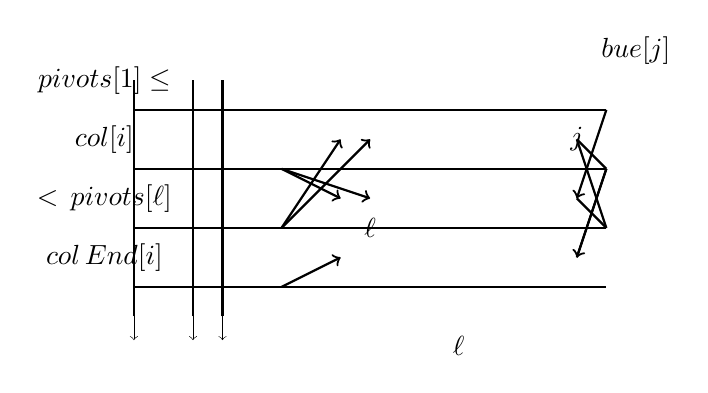
\begin{tikzpicture}[scale=0.75]
        \draw[thick] (-2.5,-0.5) -- (-2.5,3.5);
        \draw[thick] (-3,-0.5) -- (-3,3.5);
        \draw[thick] (-4,-0.5) -- (-4,3.5);
        
        \draw[thick] (-4,0) -- (4,0);
        \draw[thick] (-4,1) -- (4,1);
        \draw[thick] (-4,2) -- (4,2);
        \draw[thick] (-4,3) -- (4,3);
        
        \node at (-4.5, 3.5) {$pivots[1]\leq$};
        \node at (-4.5, 2.5) {$col[i]$};
        \node at (-4.5, 1.5) {$<\, pivots[\ell]$};
        \node at (-4.5, 0.5) {$col\,End[i]$};
        
        \node at (0,1) {$\ell$};
                
        \draw[->, thick] (-1.5,1) -- (0,2.5);   
        \draw[->, thick] (-1.5,2) -- (0,1.5);
        
        \draw[->, thick] (-1.5,0) -- (-0.5,0.5);
        \draw[->, thick] (-1.5,1) -- (-0.5,2.5);
        
        \draw[->, thick] (-1.5,2) -- (-0.5,1.5);
        
        \draw[->, thick] (4,3) -- (3.5,1.5);
        \draw[->, thick] (4,2) -- (3.5,0.5);
        
        \draw[-,thick] (4,2) -- (3.5,0.5);
        \draw[-,thick] (4,1) -- (3.5,2.5);
        
        \draw[-,thick] (4,2) -- (3.5,2.5);
        \draw[-,thick] (4,1) -- (3.5,1.5);
        
        \node at (4.5,4) {$bue[j]$};
        
        \node at (3.5,2.5) {$j$};
        
        \node at (1.5,-1) {$\ell$};
        
        \draw[->, very thin] (-2.5,-0.5) -- (-2.5,-0.9);
        \draw[->, very thin] (-3,-0.5) -- (-3,-0.9);
        \draw[->, very thin] (-4,-0.5) -- (-4,-0.9);
        
    \end{tikzpicture}
\end{center}

\end{document}